\subsection{Menu \textit{tree-view} OWL}\label{4-menu-owl}

Adicionalmente, propusemos o uso de um menu \textit{tree-view} para auxiliar na compreensão das classes OWL passíveis de serem utilizadas na anotação semântica por meio do atributo \textit{Model Reference} de SAWSDL. A representação do menu \textit{tree-view} para classes de uma ontologia OWL facilita a identificação da hierarquia entre as classes OWL. Classes de conceitos mais genéricos encontram-se mais próximas à classe na raiz da árvore enquanto que classes de conceitos mais específicos encontram-se mais próximas das folhas da árvore. No menu \textit{tree-view} OWL, todas as classes OWL são representadas, independentemente se são utilizadas em uma anotação semântica ou não.

A \figurename~\ref{fig:menu-tree-view-owl} ilustra o uso de duas classes hierarquicamente dispostas no menu \textit{tree-view}. No primeiro nível (nível 1), encontramos a classe base com um conceito mais genérico, enquanto que nos níveis inferiores (de nível 2 a nível N), encontramos as classes de conceitos mais específicos. Esta estrutura pode conter N níveis, dependendo da ontologia e a quantidade de especializações que pode existir entre suas classes.

\begin{figure}[h]
    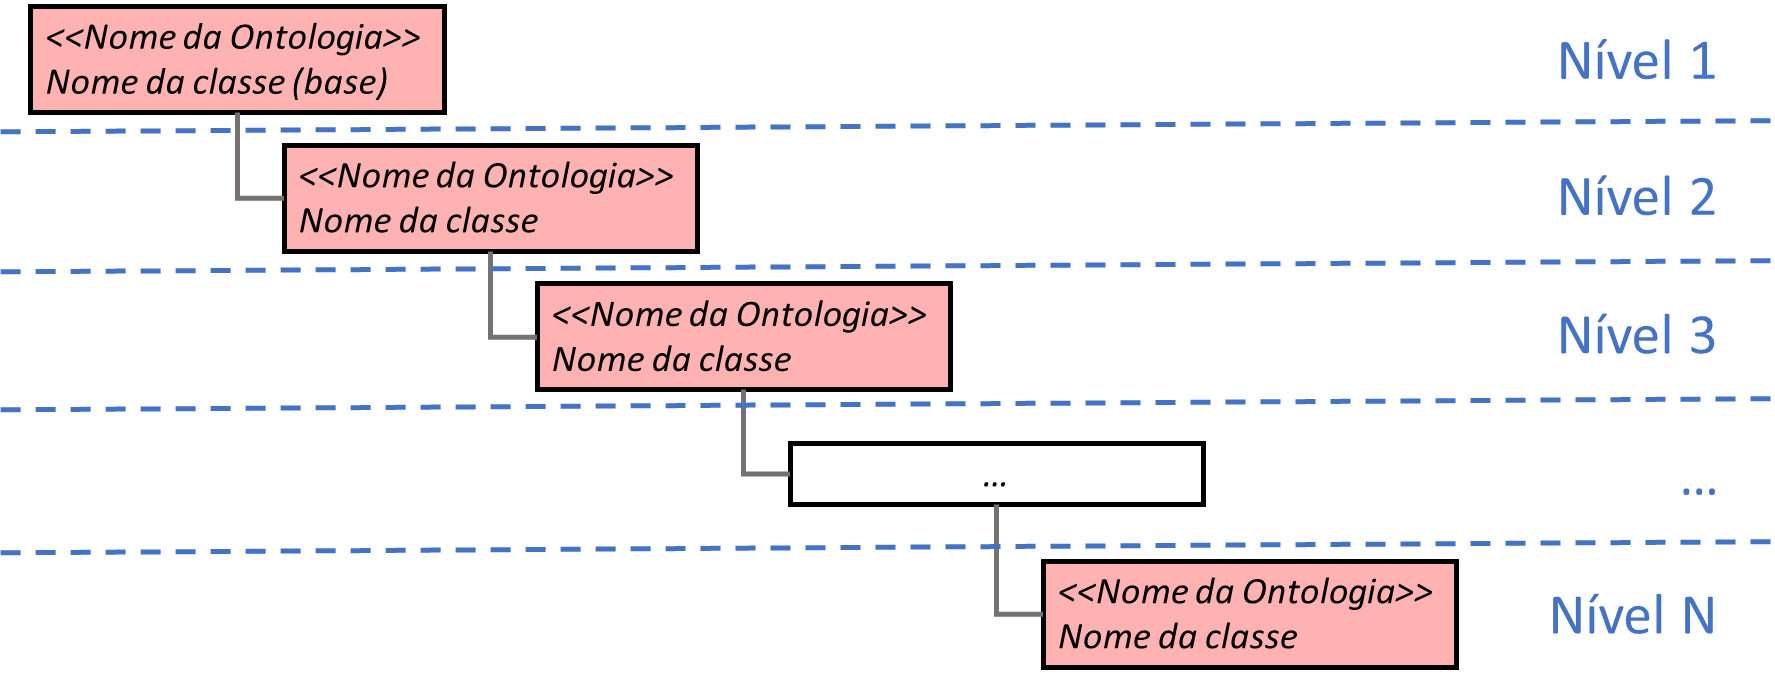
\includegraphics[scale=0.3]{4-grasews/imagens/menu-tree-view-owl.png}
    \centering
    \caption[Estrutura da representação visual do menu \textit{tree-view} para uma ontologia OWL]{\textbf{Estrutura da representação visual do menu \textit{tree-view} para uma ontologia OWL.}}
    \label{fig:menu-tree-view-owl}
\end{figure}

O menu \textit{tree-view} OWL é localizado no painel direito de Grasews. O menu \textit{tree-view} de uma ontologia OWL também provê recursos para o processo de anotação semântica por meio de um menu de contexto. Assim como no menu \textit{tree-view} WSDL, o menu de contexto do menu \textit{tree-view} OWL pode ser acessado por meio do botão direito do \textit{mouse} em uma classe OWL do menu. A \figurename~\ref{fig:grasews-menu-owl-contexto} ilustra o menu de contexto associado à classe OWL \texttt{ExpressionContext} para a anotação com o atributo \textit{Model Reference}. Neste exemplo, Grasews possibilita que um usuário adicione um URI de \texttt{ExpressionContext} como atributo \textit{Model Reference} a um elemento de uma especificação WSDL que esteja visível no grafo da ferramenta. Para adicionar uma anotação semântica \textit{Model Reference} a partir de uma classe OWL do menu \textit{tree-view}, o usuário deve selecionar o elemento WSDL/XSD no qual a anotação semântica será adicionada.

\begin{figure}[h]
    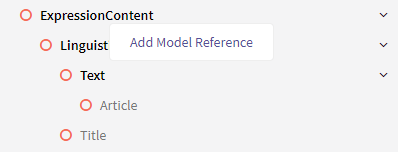
\includegraphics[scale=0.7]{4-grasews/imagens/grasews-menu-owl-contexto.png}
    \centering
    \caption[Menu de contexto para uma classe OWL no menu \textit{tree-view}]{\textbf{Menu de contexto para uma classe OWL no menu \textit{tree-view}.}}
    \label{fig:grasews-menu-owl-contexto}
\end{figure}